\chapter{Dấu fermion và các triệt tiêu siêu đối xứng}

\lectureoverview{Siêu đối xứng liên hệ boson với fermion, nhưng lý do muốn có một quan hệ như vậy dễ thấy hơn trước khi viết ra đại số của nó. Chúng ta bắt đầu từ tôpô của các phép quay, làm cho dấu của hàm sóng fermion trở nên quan sát được thông qua giao thoa, suy ra dấu âm của một vòng fermion kín từ phản đối xứng khi hoán đổi, rồi dùng các dấu vòng trái ngược nhau của boson và fermion để gợi ý sự triệt tiêu của năng lượng chân không và của tự năng vô hướng. Nửa sau đặt câu hỏi siêu đối xứng có thể bị phá vỡ nặng đến mức nào, người ta có thể phát hiện các siêu đối hạt bằng cách nào, và vì sao siêu đối xứng chính xác sẽ xóa bỏ cấu trúc lớp vỏ nguyên tử thông thường.}

\section{Trước siêu đối xứng: một điểm kỳ lạ của các phép quay}

Siêu đối xứng là một đối xứng giữa fermion và boson. Tuy nhiên, trước khi thử xây dựng nó, đáng để nhớ lại hai loại hạt này biến đổi khác nhau ra sao dưới các phép quay. Bản thân câu hỏi ấy bắt đầu từ một sự kiện tôpô dễ minh họa nhưng lại khó quên một cách đáng ngạc nhiên một khi đã thấy nó.

Đưa một bàn tay lên, lòng bàn tay ngửa, rồi xoay cổ tay một góc \(2\pi\). Bàn tay trở lại đúng hướng ban đầu, nhưng rõ ràng cánh tay chưa trở lại một cấu hình tương đương: nó bị xoắn. Tiếp tục thêm một \(2\pi\) nữa, đồng thời dịch chuyển cánh tay khi cần, thì có thể gỡ xoắn. Vì thế một phép quay \(2\pi\) không thể được biến dạng liên tục thành không quay khi môi trường xung quanh được giữ cố định, còn một phép quay \(4\pi\) thì có thể. Minh họa bằng bàn tay này là một chứng minh bằng vung tay theo đúng nghĩa đen nhất.

Cùng điểm đó có thể được nêu ra mà không cần dựa vào giải phẫu học. Đặt một quả bóng trong một chiếc hộp cố định và nối quả bóng với các thành hộp bằng một số bất kỳ các sợi dây mềm, co giãn được nhưng không thể đứt. Quay quả bóng một vòng \(2\pi\). Các sợi dây bị rối, và không chuyển động nào chỉ của riêng chúng có thể khôi phục cấu hình ban đầu. Quay quả bóng đến tổng góc \(4\pi\), và có thể luồn các sợi dây đi vòng quanh nó cho đến khi chỗ rối biến mất. Các bức tường tượng trưng cho vô cùng không gian: phép so sánh chỉ có nghĩa vì biên không bị quay cùng với quả bóng.

\begin{classroomqa}
\audiencequestion{Có thể gỡ chỗ rối đó bằng cách quay cái hộp không? \lecturetimestamp{00:02:53}}
\lecturerresponse{Như thế là thay đổi bài toán. Cái hộp biểu trưng cho vô cùng không gian và được giữ cố định. Ta đang so sánh phép quay của vật so với môi trường xung quanh nó, chứ không phải một phép quay chung của cả vật lẫn môi trường.}
\end{classroomqa}

\begin{classroomqa}
\audiencequestion{Vì sao không đơn giản quay quả bóng thêm một \(2\pi\) nữa? \lecturetimestamp{00:03:20}}
\lecturerresponse{Chính đó là điều phân biệt hai trường hợp. Nếu không quay quả bóng thêm nữa, chỗ rối để lại sau một vòng \(2\pi\) không thể gỡ được. Sau vòng thứ hai, cho tổng cộng \(4\pi\), thì có thể.}
\end{classroomqa}

Trong ngôn ngữ nhóm hiện đại, nhóm quay có hai lớp tôpô của các đường khép kín:
\begin{equation}
\pi_1\!\left(SO(3)\right)\cong \mathbb Z_2.
\end{equation}
Đi một vòng là không tầm thường, nhưng đi hai vòng thì cho lớp tầm thường.
Tương đương, \(SU(2)\) là phủ đôi của \(SO(3)\). Đây là phần tiền sử hình học của dấu fermion.

\editorialnote{Ngôn ngữ của \(SO(3)\), \(SU(2)\) và nhóm cơ bản làm cho cấu trúc tôpô trở nên tường minh. Minh họa bằng cánh tay và minh họa bằng dây xác lập cùng một tính hai trị về mặt hình học.}

\section{Phép quay \texorpdfstring{\(2\pi\)}{2 pi} tác động gì lên một trạng thái lượng tử}

Bây giờ hãy cố định vị trí của một hạt và chỉ giữ lại trạng thái spin của nó, ký hiệu là \(\ket{\psi}\). Các hạt có spin nguyên là boson và các hạt có spin bán nguyên là fermion. Một phép quay vật lý có thể được thực hiện bằng cách đặt một spin mang điện trong một từ trường mạnh rồi quay từ trường, hoặc bằng cách để spin tiến động qua góc mong muốn trong một từ trường cố định.

\begin{classroomqa}
\audiencequestion{Trong phòng thí nghiệm, spin của electron thực sự có thể bị quay như thế nào? \lecturetimestamp{00:05:26}}
\lecturerresponse{Từ trường cung cấp tay nắm để làm việc đó. Ta có thể quay một từ trường đủ mạnh để spin đi theo nó, hoặc để spin tiến động quanh một từ trường cố định. Nắm electron bằng tay không phải là một phương pháp thực nghiệm có sức cạnh tranh.}
\end{classroomqa}

Giả sử một phép quay trọn vẹn \(2\pi\) nhân trạng thái với một pha:
\begin{equation}
R(2\pi)\ket{\psi}=\xi\ket{\psi}.
\end{equation}
Thực hiện phép biến đổi ấy hai lần thì được
\begin{equation}
R(4\pi)\ket{\psi}=\xi^2\ket{\psi}.
\end{equation}
Vì đường đi \(4\pi\) là tầm thường về tôpô, nó phải tác động như toán tử đơn vị trong phép so sánh này. Do đó
\begin{equation}
\xi^2=1,
\qquad
\xi=+1\ \hbox{or}\ -1.
\end{equation}
Boson thực hiện dấu cộng còn fermion thực hiện dấu trừ:
\begin{align}
R(2\pi)\ket{\psi_B}&=+\ket{\psi_B},\\
R(2\pi)\ket{\psi_F}&=-\ket{\psi_F}.
\end{align}
Đối với một trạng thái có spin xác định \(j\), phát biểu gọn là
\begin{equation}
R(2\pi)=(-1)^{2j}.
\end{equation}
Bản chép bài giảng có nói ngắn gọn rằng khả năng thứ hai là phép nhân với \(2\pi\); phép suy dẫn xung quanh và lập luận trên bảng cho thấy rõ rằng thừa số được ngụ ý là \(-1\).

Lúc đầu điều này có vẻ không mang nội dung vật lý. Nếu toàn bộ hàm sóng đổi dấu,
\begin{equation}
\Psi\longmapsto-\Psi,
\end{equation}
thì các xác suất không đổi vì
\begin{equation}
(-\Psi)^*(-\Psi)=\Psi^*\Psi.
\end{equation}
Lấy hai tập hợp electron được chuẩn bị giống hệt nhau, quay mọi phần tử của một tập hợp đi \(2\pi\), và để tập hợp kia nguyên như cũ. Không phép đo nào trên một phần tử cô lập có thể cho biết nó đến từ tập hợp nào. Một pha toàn cục không phải là đại lượng quan sát được.

\section{Làm cho dấu âm trở thành tương đối}

Dấu trở nên quan sát được khi nó được áp đặt lên một nhánh kết hợp của hàm sóng mà không áp đặt lên nhánh kia. Cho các electron đi qua một thiết bị hai đường đi, từng hạt một. Đừng xác định đường nào được đi qua, vì thông tin đường đi sẽ phá hủy giao thoa. Gọi biên độ trên và dưới lần lượt là \(\psi_1\) và \(\psi_2\), để trạng thái sau khi ghép lại là
\begin{equation}
\Psi=\psi_1+\psi_2.
\end{equation}
Hãy tưởng tượng tạm thời giữ mỗi nhánh trong một vùng từ trường. Chỉ quay từ trường gắn với nhánh thứ hai đi \(2\pi\). Nếu hạt là một fermion, trạng thái trở thành
\begin{equation}
\Psi'=\psi_1-\psi_2.
\end{equation}
Đây không còn là một dấu toàn cục nữa. Pha tương đối làm các cực đại giao thoa dịch thành cực tiểu. Nếu hai gói trở về là ảnh gương của nhau qua giữa đầu dò, thì tổ hợp phản đối xứng triệt tiêu tại tâm:
\begin{equation}
\Psi'(0)=\psi_1(0)-\psi_2(0)=0.
\end{equation}
Vì thế electron sẽ không bao giờ được phát hiện tại điểm đối xứng ấy. Trái lại, quay cả hai nhánh sẽ cho \(-\psi_1-\psi_2=-\Psi\), điều này không có hiệu ứng quan sát được.

Bài giảng nhấn mạnh bản chất quan hệ của thí nghiệm này. Quay một vùng từ trường tương đối so với vùng kia là tương tự như quay quả bóng trong khi giữ cái hộp cố định. Quay cả hai vùng cùng nhau là tương tự như quay đồng thời quả bóng và cái hộp. Một phép quay tương đối \(4\pi\) làm mất hiệu ứng vì khi đó trạng thái fermion trở về với dấu cộng. Thí nghiệm này được Yakir Aharonov và Leonard Susskind đề xuất vào 1967 và về sau đã được thực hiện dưới dạng giao thoa kế, như bài giảng có nhắc thoáng qua. Cùng nguyên lý ấy có thể áp dụng cho electron hoặc ion mang điện: một hình vân bị dịch cho biết trạng thái spin bán nguyên, còn một hình vân không dịch cho biết trạng thái spin nguyên.

\begin{classroomqa}
\audiencequestion{Nếu từ trường tương đối bị quay đi \(4\pi\), mẫu bị dịch có trở về mẫu ban đầu không? \lecturetimestamp{00:12:21}}
\lecturerresponse{Có. Hai lần đổi dấu nhân với nhau thành \(+1\), nên pha tương đối gây ra sự hoán đổi giữa cực đại và cực tiểu biến mất.}
\end{classroomqa}

\begin{classroomqa}
\audiencequestion{Ta nên liên hệ các sợi dây trong hộp với một fermion theo nghĩa đen đến mức nào? \lecturetimestamp{00:13:43}}
\lecturerresponse{Chúng là một hình dung gợi nhớ về tôpô, không phải những sợi dây vật lý buộc vào một electron. Một boson hành xử như thể một vòng \(2\pi\) không để lại ký ức nào; một fermion giữ lại chính xác ký ức về dấu được biểu diễn bởi chỗ rối không tầm thường ấy.}
\end{classroomqa}

\begin{classroomqa}
\audiencequestion{Có phải có hai electron trong hai vùng từ trường, một hạt bị quay và hạt kia thì không? \lecturetimestamp{00:14:29}}
\lecturerresponse{Không. Chỉ có một electron trong một chồng chập không gian kết hợp. Nó có biên độ hiện diện trên một trong hai nhánh, và thiết bị không được để lộ nhánh nào nó đã đi qua. Quay một vùng làm thay đổi một biên độ tương đối với biên độ kia; quay cả hai chỉ làm thay đổi pha chung.}
\end{classroomqa}

Góc \(2\pi\) là đặc biệt vì hướng spin trở lại như cũ trong khi spinor nhận thêm một dấu. Một phép quay tương đối tổng quát cũng làm thay đổi hướng spin. Nếu hai trạng thái theo hai đường trở về với các trạng thái spin \(\ket{\chi_1}\) và \(\ket{\chi_2}\), thì hạng giao thoa tỉ lệ với
\begin{equation}
\braket{\chi_1}{\chi_2}.
\end{equation}
Độ lớn của nó chi phối độ tương phản của các vân.\editorialnote{Công thức chồng lấp spin là phần bổ sung chuẩn cho thảo luận định tính của bài giảng về sự mất giao thoa một phần và hoàn toàn.} Các trạng thái spin trực giao mang thông tin đường đi hoàn hảo và không giao thoa.

\begin{classroomqa}
\audiencequestion{Điều gì xảy ra nếu ta đo xem vùng từ trường nào chứa electron? \lecturetimestamp{00:18:03}}
\lecturerresponse{Mẫu giao thoa bị phá hủy. Bất kỳ bản ghi nào phân biệt hai đường đi đều loại bỏ sự cộng kết hợp của các biên độ của chúng.}
\end{classroomqa}

\begin{classroomqa}
\audiencequestion{Nếu mọi spin đều bắt đầu theo cùng một hướng và spin cuối cùng được đo, thì bản thân phép \(2\pi\) có làm đổi hướng đó không? \lecturetimestamp{00:18:17}}
\lecturerresponse{Không. Sau \(2\pi\), hướng spin vật lý vẫn như cũ; chỉ có nhánh fermion đã nhận một dấu âm. Đó là vì sao phép này có thể làm thay đổi giao thoa mà không để lại một hướng spin khác làm dấu mốc đường đi.}
\end{classroomqa}

\begin{classroomqa}
\audiencequestion{Nếu từ trường chỉ được quay qua \(\pi\) thay vì \(2\pi\) thì sao? \lecturetimestamp{00:18:43}}
\lecturerresponse{Khi đó hướng spin thay đổi. Một nhánh spin lên và một nhánh spin xuống là phân biệt được và không thể giao thoa. Các góc trung gian làm giảm độ tương phản một cách liên tục; một phép quay tương đối \(180^\circ\) phá hủy nó hoàn toàn.}
\end{classroomqa}

\section{Đối xứng hoán đổi và dấu của một vòng kín}

Phần thảo luận về phép quay đã tách ra một dấu âm fermion. Một dấu thứ hai, liên hệ rất gần, xuất hiện khi các hạt đồng nhất bị hoán đổi. Đối với một hàm sóng hai hạt,
\begin{align}
P_{12}\Psi_B(1,2)&=+\Psi_B(1,2)=+\Psi_B(2,1),\\
P_{12}\Psi_F(1,2)&=-\Psi_F(1,2)=-\Psi_F(2,1).
\end{align}
Các trạng thái boson là đối xứng còn các trạng thái fermion là phản đối xứng.

\begin{figure}[htbp]
\centering
\includegraphics[width=0.74\textwidth]{lecture_02_figure_02.png}
\lectureframe{00:24:27}
\caption{Lập luận hoán đổi trong ký pháp trạng thái. Chỉ nhãn ket là đọc được một cách chắc chắn trong khung hình; các phương trình phản đối xứng được đánh máy trong văn bản thay vì quy cho phần phấn viết bị che khuất.}
\end{figure}

Bây giờ ta có thể xác định dấu tương đối của một vòng hạt kín mà không cần tính tích phân của nó. Hãy xét một biểu đồ Feynman chân không không có chân ngoài. Nó có thể được hình dung như một hạt vạch ra một đường khép kín trong không-thời gian, hoặc như một cặp hạt-phản hạt được tạo ra rồi sau đó hủy nhau. Một biểu đồ chân không như vậy đóng góp vào biên độ chân không và do đó vào năng lượng chân không.

Hãy bắt đầu với hai bản sao tách rời của vòng. Các biểu đồ rời nhau nhân với nhau, nên nếu một vòng có dấu \(\sigma\) thì cặp đó có dấu
\begin{equation}
\sigma^2=+1.
\end{equation}
Cắt cả hai vòng tại cùng một thời điểm, chẳng hạn \(t=0\). Trên lát cắt đó có hai hạt đồng nhất. Nối lại chúng mà không hoán đổi thì hai vòng riêng rẽ quay trở lại. Hoán đổi hai hạt trước khi nối lại thì tôpô trở thành một vòng. Phép hoán đổi đóng góp \(+1\) cho boson và \(-1\) cho fermion. Vì dấu ban đầu của hai vòng là dương, nên các dấu một vòng thu được là
\begin{equation}
\begin{aligned}
\operatorname{sign}(\text{closed boson loop})&=+1,\\
\operatorname{sign}(\text{closed fermion loop})&=-1.
\end{aligned}
\end{equation}
Tổng quát hơn, một biểu đồ có \(L_F\) vòng fermion kín độc lập mang thừa số
\begin{equation}
(-1)^{L_F}.
\end{equation}
Bài giảng cố ý suy ra quy tắc này từ phép hoán đổi thay vì viện đến phép tích phân Grassmann. Lập luận sơ cấp này làm lộ rõ nguồn gốc vật lý của dấu.

\section{Dấu vòng đối nhau và năng lượng chân không}

Một vòng chân không boson làm tăng đóng góp năng lượng chân không với một dấu, còn một vòng fermion đóng góp với dấu ngược lại. Điều này lập tức gợi ý một hướng suy nghĩ, vì mật độ năng lượng tối quan sát được là cực kỳ nhỏ so với các ước lượng ngây thơ dùng ngưỡng cắt trong lý thuyết trường lượng tử. Bài giảng nêu độ chênh khét tiếng này là cỡ \(123\) bậc độ lớn. Số mũ chính xác còn tùy vào thang tử ngoại nào được dùng; điểm cốt lõi bền vững là sự vênh nhau khổng lồ ấy.

Đóng góp của một vòng không chỉ phụ thuộc vào thống kê. Nó phụ thuộc vào khối lượng, điện tích, độ bội và các tương tác. Tuy nhiên, nếu một boson và một fermion trùng khớp về mọi tính chất liên quan, thì các đóng góp có độ lớn bằng nhau của chúng có thể triệt tiêu lẫn nhau:
\begin{equation}
\begin{gathered}
m_B=m_F,\qquad q_B=q_F,\qquad g_B=g_F,\\
\Delta\rho_{\mathrm{vac}}^{(B)}
+\Delta\rho_{\mathrm{vac}}^{(F)}=0.
\end{gathered}
\end{equation}
Nhận xét này không giải quyết được bài toán hằng số vũ trụ học. Nó chỉ cung cấp điều mà bản thân các vòng boson thông thường không thể cung cấp: các đóng góp trái dấu. Trong một lý thuyết siêu đối xứng toàn cục với siêu đối xứng hoàn toàn không bị phá vỡ, sự triệt tiêu năng lượng chân không quả thật có thể là chính xác dưới những giả thiết thích hợp; sau khi siêu đối xứng bị phá vỡ, giá trị nhỏ bé nhưng khác không được quan sát vẫn chưa được giải thích.\editorialnote{Sự bảo lưu này tách động cơ của bài giảng khỏi bài toán hằng số vũ trụ học khó hơn nhiều.}

Ta đã biết rằng sự khớp đúng tuyệt đối không mô tả tự nhiên. Nếu electron có một đối tác spin-0 với cùng khối lượng và điện tích, thì sự hủy electron-positron qua một photon ảo có thể tạo ra một cặp như vậy:
\begin{equation}
e^-e^+\longrightarrow\gamma^*
\longrightarrow\widetilde e^-\widetilde e^+.
\end{equation}
Một hạt vô hướng mang điện suy biến như thế đã không thể thoát khỏi các thí nghiệm máy va chạm thông thường. Vì vậy, phép phản chiếu boson-fermion không thể là một đối xứng chính xác của phổ quan sát được. Đây là sự phản chiếu trong loại hạt, không phải sự phản chiếu trong không gian vật lý.

\section{Mục tiêu trước mắt hơn: tự năng lượng của trường vô hướng}

Năng lượng chân không là minh họa đầu tiên, nhưng mối quan tâm chính của bài giảng là tính bất ổn bức xạ của khối lượng các trường vô hướng. Một trường vô hướng ban đầu có khối lượng trần bằng 0 có thể nhận một hiệu chỉnh nhạy với ngưỡng cắt theo bậc hai. Về sơ đồ,
\begin{equation}
\Delta m_H^2\sim \frac{g_B^2}{16\pi^2}\Lambda^2
\end{equation}
từ một vòng boson. Khối lượng fermion có một cơ chế bảo vệ khác: khi một fermion không khối lượng có đối xứng chiral chính xác, các hiệu chỉnh bức xạ không thể sinh ra một hạng khối lượng cộng thêm. Đó chính là lập luận trái-phải của bài giảng trước.

Bây giờ hãy hình dung một đối xứng đủ chặt chẽ để đặt một trường vô hướng và một fermion vào cùng một đa bội và làm khớp các tương tác của chúng. Khi đó xuất hiện một vòng fermion với dấu ngược lại:
\begin{equation}
\Delta m_H^2
\sim
\frac{g_B^2-g_F^2}{16\pi^2}\Lambda^2+\cdots .
\end{equation}
Nếu siêu đối xứng áp đặt \(g_B=g_F\) và các khối lượng bằng nhau, thì các hạng bậc hai triệt tiêu nhau. Nhờ đó, sự bảo vệ của fermion được truyền sang đối tác boson của nó. Đây không chỉ là một sự trùng hợp số học giữa hai biểu đồ; đối xứng phải cưỡng bức sự triệt tiêu qua mọi bậc và mọi tương tác được phép.

Phép so sánh trải rộng trên bảng cho thấy bài giảng chuyển từ các vòng riêng lẻ sang các hiệu chỉnh vòng ghép cặp của các hạt lan truyền.

\begin{figure}[htbp]
\centering
\includegraphics[width=0.79\textwidth]{lecture_02_figure_04.png}
\lectureframe{00:40:23}

\medskip
\begin{tikzpicture}[scale=0.9]
\draw (-4.2,0) circle (0.55);
\draw[dashed] (-2.4,0) circle (0.55);
\draw (0,0) -- (3.7,0);
\fill (1.85,0) circle (0.055);
\draw (1.85,0) -- (1.85,0.25);
\draw[dashed] (1.85,0.85) circle (0.6);
\end{tikzpicture}
\caption{So sánh trên toàn bảng giữa các tôpô vòng thông thường và tôpô vòng của hạt đối tác. Bản phác thảo đánh máy chỉ giữ lại sự tương phản tôpô có thể nhìn thấy; nó không gán các nhãn hạt bị che khuất.}
\end{figure}

Sau giờ nghỉ trong lớp, lập luận được khởi động lại bằng cái được gọi là bức tranh bậc không. Đây không phải là một bậc trong lý thuyết nhiễu loạn. Nó có nghĩa là cách mô tả hữu ích thô nhất:
\begin{quote}
Với mỗi hạt đều có một siêu đối tác mang thống kê ngược lại. Mọi fermion đều có một đối tác boson, và mọi boson đều có một đối tác fermion.
\end{quote}
Trong một lý thuyết siêu đối xứng chính xác, các đối tác ấy cũng sẽ suy biến, nghĩa là có cùng khối lượng. Tự nhiên không suy biến theo cách đó. Dù vậy, nếu các khối lượng không bằng nhau nhưng không quá cách xa, thì sự triệt tiêu vẫn có thể đủ tốt để ngăn một hiệu chỉnh vô hướng lớn đến mức bùng nổ. Với sự phá vỡ siêu đối xứng mềm, thang nguy hiểm được thay thế một cách sơ đồ bởi độ tách khối lượng của siêu đối tác:
\begin{equation}
\Delta m_H^2\sim
\frac{g^2}{16\pi^2}\,\Delta m_{\mathrm{SUSY}}^2
\ln\!\frac{\Lambda^2}{\Delta m_{\mathrm{SUSY}}^2}
\end{equation}
cho tới các hệ số phụ thuộc mô hình.\editorialnote{Công thức này diễn đạt phát biểu định tính của bài giảng rằng sự khớp khối lượng không hoàn hảo để lại một hiệu chỉnh còn dư do độ tách chi phối; nó không được chép từ trên bảng.}

\section{Siêu đối xứng bị phá vỡ và canh bạc thực nghiệm năm 2010}

Khi bài giảng này được ghi lại vào 2010, chưa có siêu đối tác nào được quan sát. Suy luận trực tiếp khi đó là nếu chúng có thật thì chúng phải nặng hơn các hạt đã biết và vượt quá tầm với của các máy trước đó. Các mô hình siêu đối xứng cũng phân biệt các hạt có khối lượng chỉ phát sinh sau khi đối xứng điện yếu bị phá vỡ với các trạng thái được phép mang những khối lượng lớn hơn mà vẫn bảo toàn đối xứng. Bài giảng nêu điều này như một cơ sở lý giải vì sao nửa nhìn thấy của một phổ siêu đối xứng có thể nhẹ còn nửa chưa thấy thì nặng hơn, đồng thời thẳng thắn gọi cách sắp xếp ấy là hơi gượng ép. Susskind nêu kỳ vọng riêng của mình rằng các siêu đối tác sẽ được phát hiện, rồi lập tức đánh dấu đó là một phỏng đoán chứ không phải một kết quả.

Do đó, Máy Va chạm Hadron Lớn giữ vai trò trung tâm trong viễn cảnh của bài giảng. Người ta kỳ vọng nó sẽ tìm kiếm cả boson Higgs lẫn các siêu đối tác. Những phát biểu này phải được đọc trong bối cảnh 2010 của chúng: bài giảng đang giải thích canh bạc thực nghiệm trước khi có phát hiện Higgs và trước các kết quả tìm kiếm sau này của LHC.

Vì sao một siêu đối tác được thúc đẩy bởi tính tự nhiên lại không nên nằm ở thang Planck? Vì khi đó nó sẽ thất bại trong nhiệm vụ được giao cho nó. Nếu khối lượng boson và fermion chênh nhau quá lớn, các tích phân vòng của chúng ngừng triệt tiêu nhau phía trên khối lượng nhẹ hơn. Hiệu chỉnh vô hướng còn dư khi ấy được ấn định xấp xỉ bởi độ tách lớn đó chứ không phải bởi thang yếu. Siêu đối xứng ở một thang xa tùy ý vẫn là một đối xứng toán học, nhưng nó không còn mang lại một lời giải thích thuyết phục cho một sector Higgs nhẹ.

Bài giảng chuyển điều này thành kỳ vọng của thời đó rằng các độ tách liên quan nên nằm trong khoảng cỡ vài trăm GeV và vì thế trong tầm với của LHC. Ước lượng số này mang tính lịch sử và phụ thuộc mô hình; chuỗi logic mới quan trọng hơn:
\begin{equation}
\begin{gathered}
\text{Higgs protection}\\
\Downarrow\\
\text{effective boson--fermion cancellation}\\
\Downarrow\\
\Delta m_{\mathrm{SUSY}}\ \text{not too large}.
\end{gathered}
\end{equation}

\begin{classroomqa}
\audiencequestion{Liệu mọi đóng góp fermion có thể chỉ đơn thuần triệt tiêu mọi đóng góp boson một cách gộp chung, mà không cần các đối tác một-một? \lecturetimestamp{00:45:01}}
\lecturerresponse{Chúng có thể triệt tiêu nhau về mặt số học, nhưng khi đó đó sẽ là một sự triệt tiêu ngẫu nhiên được tinh chỉnh chẳng kém gì bài toán ban đầu. Đề xuất siêu đối xứng mạnh hơn ở chỗ: những giả thiết hợp lý cưỡng bức các đóng góp khớp nhau, còn siêu đối xứng bị phá vỡ giải thích vì sao các khối lượng chỉ khớp xấp xỉ. Năng lượng chân không là minh họa; mối quan tâm trực tiếp ở đây là tự năng lượng Higgs.}
\end{classroomqa}

\begin{classroomqa}
\audiencequestion{Việc gọi một sự triệt tiêu gộp chung là không tự nhiên có phải đã ngầm giả định một cách tổ chức lý thuyết theo hướng quy giản luận không? \lecturetimestamp{00:47:51}}
\lecturerresponse{Đó là một chất vấn xác đáng. Không ai có một định nghĩa cuối cùng về tính tự nhiên, và việc tìm kiếm phần nào là sự lần mò để tìm một lời giải thích có sức thuyết phục. Siêu đối xứng và sự phá vỡ siêu đối xứng tự phát cung cấp những khuôn khổ toán học đã biết có thể cưỡng bức mẫu hình mong muốn. Những câu hỏi chưa được giải quyết là liệu tự nhiên có dùng khuôn khổ đó hay không, và liệu nó có phải là duy nhất hay không.}
\end{classroomqa}

\section{Sản sinh trực tiếp, hiệu ứng ảo và chuỗi phân rã}

Một hạt nặng không nhất thiết phải được tạo ra trên vỏ khối lượng mới ảnh hưởng đến một thí nghiệm. Nó có thể xuất hiện ảo bên trong một vòng và sửa đổi nhẹ một biên độ tán xạ electron-positron thông thường. Vì vậy, các phép đo điện yếu chính xác vẫn ràng buộc các siêu đối tác ngay cả khi năng lượng trong hệ tâm khối nằm dưới ngưỡng sản sinh cặp trực tiếp
\begin{equation}
\sqrt{s}<2m_{\widetilde p}.
\end{equation}
Đánh giá của bài giảng vào 2010 là dữ liệu chính xác khi ấy đã siết chặt không gian tham số siêu đối xứng nhưng chưa loại trừ nó.

\begin{classroomqa}
\audiencequestion{Liệu có thể suy ra gián tiếp các siêu đối tác, giống như trước đây các hạt nặng từng bị ràng buộc thông qua các suất tạo chính xác trước khi được quan sát trực tiếp không? \lecturetimestamp{00:49:01}}
\lecturerresponse{Có. Một vòng siêu đối tác ảo làm thay đổi nhẹ một biên độ thông thường, nên vấn đề trở thành hiện tượng học điện yếu độ chính xác cao chứ không phải sản sinh trực tiếp. Một máy va chạm electron-positron sạch và đủ năng lượng sẽ đặc biệt hữu ích. Các va chạm proton lộn xộn hơn vì proton là một trạng thái hợp thành của quark và gluon; trên thực tế người ta va chạm các thành phần dao động, chứ không phải hai hạt sơ cấp với điều kiện đầu được biết sắc nét.}
\end{classroomqa}

Một sinh viên hỏi về việc xét phản ứng theo chiều ngược lại, bắt đầu từ nhiều siêu hạt sẵn có. Trở ngại không phải là đối xứng đảo thời gian mà là tính sẵn có. Các siêu đối tác nặng trước hết phải được tạo ra, và đa số được kỳ vọng sẽ phân rã nhanh thành các trạng thái nhẹ hơn.

\begin{classroomqa}
\audiencequestion{Nếu một vũ trụ chứa nhiều siêu hạt, liệu hai hạt trong số đó có thể va chạm và biến thành các hạt thông thường không? \lecturetimestamp{00:53:43}}
\lecturerresponse{Về nguyên tắc, các phản ứng liên quan có những kênh nghịch, nhưng các siêu đối tác nặng không được kỳ vọng sẽ còn tồn tại tự do với số lượng dồi dào. Chúng phân rã về các trạng thái năng lượng thấp hơn, nên trước hết một thí nghiệm phải cung cấp đủ năng lượng va chạm để tạo ra chúng.}
\end{classroomqa}

Điều này dẫn tới câu hỏi về vật chất tối. Trong nhiều mô hình siêu đối xứng, một quy tắc chọn rời rạc ngăn siêu đối tác cuối cùng trong một chuỗi phân rã biến mất hoàn toàn. Khi đó, mọi siêu đối tác nặng hơn đều phân rã dây chuyền xuống siêu đối tác nhẹ nhất, hay LSP. Nếu LSP trung hòa điện, nó có thể bền và khó phát hiện, khiến nó trở thành một ứng viên khả dĩ cho vật chất tối. Bản chép có một chỗ nói "năng lượng tối" trong đoạn trao đổi này, nhưng câu hỏi của người nghe và mô tả về hạt đều cho thấy rõ ràng rằng chủ đề ở đây là vật chất tối.

\begin{classroomqa}
\audiencequestion{Việc siêu đối tác phân rã nhanh có mâu thuẫn với đề xuất rằng một siêu đối tác có thể là vật chất tối không? \lecturetimestamp{00:54:53}}
\lecturerresponse{Không. Phần lớn các siêu đối tác có thể phân rã trong khi hạt nhẹ nhất vẫn ổn định trong những mô hình đòi hỏi một siêu đối tác ở cuối mỗi chuỗi phân rã. Điện tích nói chung làm nảy sinh thêm những khó khăn hiện tượng học, nên LSP khả dĩ nhiều khả năng là trung hòa. Về nguyên tắc nó không phải là không thể phát hiện, nhưng nó sẽ không để lại vệt ion hóa hiển nhiên như một selectron mang điện.}
\end{classroomqa}

\section{Khớp có nghĩa là phải khớp cả các hằng số ghép}

Chỉ khớp khối lượng thôi thì chưa đủ. Hãy so sánh một vòng chân không electron với một vòng selectron. Thống kê đối ngược của chúng cho dấu đối ngược, nhưng để có cùng độ lớn thì cần khối lượng bằng nhau. Bây giờ gắn thêm hai photon ngoài. Các hệ số cũng chứa các hằng số ghép điện, nên sự triệt tiêu đòi hỏi điện tích bằng nhau:
\begin{equation}
\begin{gathered}
q_{\widetilde e}=q_e,\\
\mathcal A_{\mathrm{loop}}^{(e)}
+\mathcal A_{\mathrm{loop}}^{(\widetilde e)}=0,\\
\text{provided the full couplings match.}
\end{gathered}
\end{equation}
Bất kỳ sự không khớp nào ở bất kỳ mức nào đều để lại một hạng phân kỳ chưa bị triệt tiêu. Siêu đối xứng có giá trị vì nó liên hệ cả các tương tác, chứ không chỉ tên gọi và spin.

\begin{figure}[H]
\centering
\includegraphics[width=0.66\textwidth]{lecture_02_figure_05.png}
\lectureframe{00:57:15}

\medskip
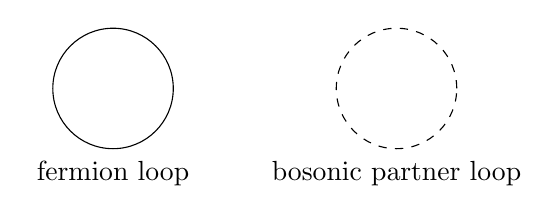
\begin{tikzpicture}[scale=0.9]
\draw (-2.0,0) circle (0.85);
\draw[dashed] (2.0,0) circle (0.85);
\node at (-2.0,-1.2) {fermion loop};
\node at (2.0,-1.2) {bosonic partner loop};
\end{tikzpicture}
\caption{Các vòng nét liền và nét đứt được so sánh trong lập luận về sự khớp điện tích. Các dấu ngoài bị cắt xén không được phục dựng, vì chỉ riêng khung hình không xác định được mọi chỗ gắn.}
\end{figure}

\begin{classroomqa}
\audiencequestion{Liệu các siêu đối tác có thể đã thoát khỏi sự phát hiện chỉ đơn giản vì các hằng số ghép của chúng khác nhau không? \lecturetimestamp{00:56:23}}
\lecturerresponse{Không, nếu các biểu đồ giống nhau được kỳ vọng sẽ triệt tiêu nhau. Thêm các tương tác photon vào sẽ kiểm tra điện tích của từng đường. Các hằng số ghép không bằng nhau cho các thừa số vòng số học không bằng nhau và khôi phục phần dư lớn. Đối xứng phải làm khớp các điện tích và tương tác thích hợp.}
\end{classroomqa}

\begin{classroomqa}
\audiencequestion{Siêu đối tác của photon cũng phải không có khối lượng sao? \lecturetimestamp{00:58:01}}
\lecturerresponse{Trong một lý thuyết siêu đối xứng chính xác, nó sẽ không có khối lượng vì nó sẽ suy biến với photon. Thế giới quan sát được không siêu đối xứng một cách chính xác, nên một trạng thái vật lý kiểu photino không nhất thiết phải có cùng khối lượng với photon.}
\end{classroomqa}

\section{Từ điển siêu đối tác}

Các quy tắc đặt tên không thanh nhã nhưng hữu ích. Một boson nhận một đối tác fermion mà tên thường kết thúc bằng \emph{-ino}: photon và photino, hạt \(W\) và wino, hạt \(Z\) và zino, gluon và gluino, Higgs và Higgsino, graviton và gravitino. Một fermion thông thường nhận một đối tác boson mà tên thường bắt đầu bằng \emph{s-}: electron và selectron, quark và squark.

\begin{center}
\begin{tabular}{@{}>{\raggedright\arraybackslash}p{0.40\linewidth}>{\raggedright\arraybackslash}p{0.52\linewidth}@{}}
\toprule
trạng thái thông thường & siêu đối tác và độ thay đổi spin\\
\midrule
Higgs vô hướng, \(j=0\) & Higgsino, \(j=\tfrac12\); \(\Delta j=+\tfrac12\)\\
boson chuẩn, \(j=1\) & gaugino, \(j=\tfrac12\); \(\Delta j=-\tfrac12\)\\
fermion vật chất, \(j=\tfrac12\) & sfermion, \(j=0\); \(\Delta j=-\tfrac12\)\\
graviton, \(j=2\) & gravitino, \(j=\tfrac32\); \(\Delta j=-\tfrac12\)\\
\bottomrule
\end{tabular}
\end{center}

Quan hệ tổng quát là các thành viên của một siêu bội khác nhau nửa đơn vị spin:
\begin{equation}
\Delta j=\frac12.
\end{equation}
Các ví dụ phác thảo trong bài giảng ghép một fermion vật chất spin-\(\tfrac12\) với một hạt vô hướng, và một boson chuẩn spin-một với một gaugino spin-\(\tfrac12\). Một mô hình tương tác hoàn chỉnh có thể trộn các trạng thái sau khi đối xứng bị phá vỡ, nên các trạng thái riêng khối lượng vật lý không nhất thiết giữ lại những tên gọi đơn giản nhất này.

\begin{classroomqa}
\audiencequestion{Liệu tất cả các đối tác vô hướng mới đều có thể tự mình trải qua sự phá vỡ đối xứng tự phát hay không? \lecturetimestamp{01:01:27}}
\lecturerresponse{Các trường vô hướng có thể nhận giá trị kỳ vọng, nhưng việc có thêm những sự phá vỡ đối xứng tùy tiện sẽ là thảm họa về mặt hiện tượng học. Một mô hình siêu đối xứng khả dĩ phải sắp xếp thế vô hướng của nó sao cho màu, điện tích, và các đối xứng cần thiết khác không bị phá vỡ theo cách sai.}
\end{classroomqa}

\begin{classroomqa}
\audiencequestion{Higgsino có những tương tác đặc biệt tương ứng với hạng tử quartic của Higgs không? \lecturetimestamp{01:02:19}}
\lecturerresponse{Siêu đối xứng ghép khớp các tương tác cũng như các hạt. Quan hệ này không thu được bằng cách ngây thơ thay mọi đường Higgs bằng một đường Higgsino, nhưng hạng tử quartic vô hướng cùng các tương tác fermion và phụ trợ liên quan cùng nằm trong một cấu trúc bị ràng buộc. Những chi tiết đó vẫn chưa được triển khai trong bài giảng.}
\end{classroomqa}

\begin{classroomqa}
\audiencequestion{Định lý quay \(2\pi\) so với \(4\pi\) có những phiên bản tương tự trong các số chiều khác không? \lecturetimestamp{01:03:07}}
\lecturerresponse{Có, nhưng số chiều làm thay đổi các khả năng. Trong hai chiều không gian, các đường đi trao đổi có thể quấn quanh nhau, cho phép các anyon có pha trao đổi tổng quát hơn \(+1\) của boson và \(-1\) của fermion. Những kích thích như vậy xuất hiện trong các hệ vật chất ngưng tụ, nhưng chúng nằm ngoài lộ trình của học phần hiện tại.}
\end{classroomqa}

\section{Vì sao siêu đối xứng chính xác sẽ xóa bỏ hóa học}

Cuối cùng, ta hỏi một thế giới siêu đối xứng chính xác sẽ như thế nào. Ở đây, tính chính xác có nghĩa là khối lượng bằng nhau và các tương tác khớp nhau cho mọi cặp hạt-siêu đối tác. Electron sẽ có một selectron boson với cùng khối lượng và điện tích, còn photon không khối lượng sẽ có một photino fermion không khối lượng:
\begin{equation}
m_{\widetilde e}=m_e,
\qquad
q_{\widetilde e}=q_e,
\qquad
m_{\widetilde\gamma}=m_\gamma=0.
\end{equation}

Cấu trúc tuần hoàn quen thuộc của hóa học phụ thuộc vào thống kê Fermi. Hiđrô có một electron ở orbital thấp nhất của nó. Heli chứa được hai electron ở đó vì các nhãn spin khác nhau. Electron thứ ba của liti buộc phải chiếm một orbital cao hơn: nguyên lý loại trừ Pauli ngăn ba electron đồng nhất chiếm cùng một trạng thái một hạt. Electron ngoài cùng đó có năng lượng lớn hơn và có xu hướng rơi vào trong, thông thường bằng cách phát ra một photon, nhưng các trạng thái thấp hơn đã lấp đầy chặn chuyển tiếp này.

Siêu đối xứng chính xác mở ra một kênh khác:
\begin{equation}
e^-_{\mathrm{outer}}
\longrightarrow
\widetilde e^-_{\mathrm{inner}}
+
\widetilde\gamma .
\end{equation}
Electron ban đầu và photino phát ra là fermion, còn selectron còn lại là boson. Vì selectron tuân theo thống kê Bose chứ không phải thống kê Fermi, hạt ở trạng thái cuối không bị cấm chiếm một orbital thấp đã có hạt ở sẵn. Vì thế electron hóa trị có thể chuyển hóa theo kênh ấy và rơi vào trong.

\begin{figure}[H]
\centering
\includegraphics[width=0.62\textwidth]{lecture_02_figure_06.png}
\lectureframe{01:09:18}

\medskip
\begin{tikzpicture}[scale=0.9]
\fill (0,0) circle (0.075);
\draw (0,0) circle (0.72);
\draw (0,0) circle (1.45);
\draw[-{Latex[length=2.2mm]}] (1.42,0.2) .. controls (1.2,0.52) and (0.92,0.42) .. (0.72,0.1);
\draw[decorate,decoration={snake,amplitude=1.4pt,segment length=7pt},-{Latex[length=2.2mm]}]
  (1.58,0) -- (3.55,0);
\node[above] at (2.7,0.12) {$\widetilde\gamma$};
\node[below] at (0,-1.65) {selectron drops to a lower orbital};
\end{tikzpicture}
\caption{Chuyển tiếp nguyên tử được dùng để cho thấy vì sao siêu đối xứng chính xác sẽ làm thay đổi hóa học. Đường lượn sóng đi ra được vẽ thấy rõ; việc nhận diện nó là một photino đến từ bản ghi chép.}
\end{figure}

Điểm này không chỉ giới hạn ở một nguyên tử kiểu liti. Trong một nguyên tử lớn, các electron hóa trị là thứ tạo ra sự đa dạng hóa học. Nếu chúng có thể liên tiếp chuyển thành các selectron boson, chúng có thể dồn vào vùng thấp nhất còn khả dụng về năng lượng thay vì lấp đầy các lớp vỏ. Kết quả sẽ giống một quần thể boson tập trung gần hạt nhân, chứ không phải cấu trúc quen thuộc của các orbital hóa trị. Những phân tử được tạo nên từ các liên kết định hướng và các lớp vỏ lấp đầy một phần sẽ không còn tồn tại dưới dạng có thể nhận ra. Bài giảng gọi hậu duệ liti giả định ấy là \emph{slithium}, nhưng trò đùa này mang theo một kết luận nghiêm túc: siêu đối xứng chính xác sẽ tạo ra vật chất không giống hóa học thông thường, và vì thế cũng không giống sinh học thông thường.

\begin{classroomqa}
\audiencequestion{Liệu chuyển tiếp electron-thành-selectron có thể ghép yếu đến mức các nguyên tử thông thường vẫn tồn tại không? \lecturetimestamp{01:10:23}}
\lecturerresponse{Không, không phải trong lý thuyết chính xác đang được hình dung. Siêu đối xứng liên hệ chuyển tiếp ấy với tương tác điện từ, nên hằng số ghép của nó được cố định bởi điện tích chứ không thể tự do chọn cho nhỏ xíu. Bài giảng đưa ra một ước lượng thô cho thời gian sống cỡ một micro giây của một nguyên tử kiểu liti, không phải như một phép tính chính xác mà để nhấn mạnh rằng sự phân rã sẽ nhanh.}
\end{classroomqa}

Vì thế, từ vật chất thường ngày, hoàn toàn tách biệt với các tìm kiếm tại máy va chạm, ta biết rằng siêu đối xứng không thể chính xác ở năng lượng thấp. Độ chênh giữa khối lượng của hạt và siêu đối tác là khổng lồ so với các thang nguyên tử hoặc proton, ngay cả nếu nó nhỏ xíu so với thang thống nhất hoặc thang Planck.

\begin{classroomqa}
\audiencequestion{Vậy thì, tại sao siêu đối xứng lại bị phá vỡ? \lecturetimestamp{01:11:19}}
\lecturerresponse{Bài giảng đưa ra một phát biểu chọn lọc tối thiểu: nếu nó không bị phá vỡ, các quan sát viên được cấu thành từ hóa học thông thường sẽ không hiện diện để đặt câu hỏi ấy. Điều đó không thay thế cho một lý thuyết động lực học về sự phá vỡ siêu đối xứng. Nó chỉ giải thích vì sao một thế giới năng lượng thấp siêu đối xứng chính xác không thể là thế giới của chúng ta.}
\end{classroomqa}

Việc phá vỡ siêu đối xứng là khả dĩ về mặt toán học và trong nhiều cách xây dựng thì khá phổ biến, dù việc sắp đặt một sự phá vỡ hiện thực còn lâu mới tự động. Ngược lại, các lý thuyết trường lượng tử siêu đối xứng chính xác sở hữu đủ cấu trúc đặc biệt để một số trong chúng có thể được phân tích sâu hơn rất nhiều so với các lý thuyết tổng quát. Chúng vừa đóng vai trò là những ứng viên để tổ chức vật lý hạt, vừa là những phòng thí nghiệm toán học mạnh mẽ một cách khác thường. Bài giảng tiếp theo sẽ chuyển từ động cơ vật lý này sang nhiều hơn trong số các cấu trúc ấy.

\section{Mạch lập luận}

Con đường đi tới siêu đối xứng đã được cố ý chọn là gián tiếp:
\begin{enumerate}
\item Phép quay không gian \(2\pi\) thuộc một lớp tôpô không tầm thường, còn phép quay \(4\pi\) có thể biến dạng liên tục về đồng nhất.
\item Trạng thái fermion nhận một dấu trừ dưới \(2\pi\), và một thí nghiệm hai đường đi làm cho dấu ấy quan sát được khi nó là tương đối chứ không phải toàn cục.
\item Tính phản đối xứng của fermion dưới phép trao đổi cho mỗi vòng fermion kín một dấu trừ bổ sung so với một vòng boson.
\item Các dấu vòng lặp đối nhau cho phép các sự triệt tiêu do đối xứng áp đặt của các đóng góp chân không và tự năng vô hướng khi khối lượng và hằng số ghép khớp nhau.
\item Sự khớp chính xác không có trong tự nhiên. Nếu siêu đối xứng bảo vệ ngành Higgs, thì sự phá vỡ của nó không thể làm các đối tác liên quan nặng một cách tùy ý.
\item Siêu đối xứng năng lượng thấp chính xác sẽ cho phép electron chuyển thành các selectron boson và làm sụp đổ cấu trúc lớp vỏ mà hóa học thông thường dựa vào.
\end{enumerate}

Vì thế, siêu đối xứng vừa hấp dẫn vừa bất khả trong dạng chính xác ngây thơ của nó vì cùng một lý do: nó ràng buộc boson và fermion với nhau một cách chặt chẽ. Quan hệ chặt chẽ ấy có thể kiềm chế những hiệu chỉnh lượng tử nguy hiểm, nhưng nếu nó tồn tại nguyên vẹn xuống tới vật lý nguyên tử, thế giới sẽ không còn giống thế giới quanh ta nữa.
